\subsection{实验目的}
理解遥感图像目标检测的概念,根据实验七中完成的实验数据,即二值检测结果,完成检测结果的后处理。包括连通分量提取与分析,目标像素聚类,以及目标切片的提取与显示等。
\subsection{实验原理}
\subsubsection{目标检测的一般流程}
\begin{figure}[H]
	\centering
	\begin{tikzpicture}[node distance=4cm]
	\node[process](raw_rs_img){原始遥感图像};
	\node[process, right of=raw_rs_img](binary_img){二值检测结果图像};
	\node[process, right of=binary_img](abstract_obj){候选目标提取};
	\node[process, right of=abstract_obj](remove_false_alert){虚警去除};
	
	\draw[->] (raw_rs_img) -- (binary_img);
	\draw[->] (binary_img) -- (abstract_obj);
	\draw[->] (abstract_obj) -- (remove_false_alert);
	\end{tikzpicture}
\end{figure}
\subsubsection{连通分量的提取}
\begin{figure}[H]
	\centering
	\begin{minipage}{0.45\linewidth}
		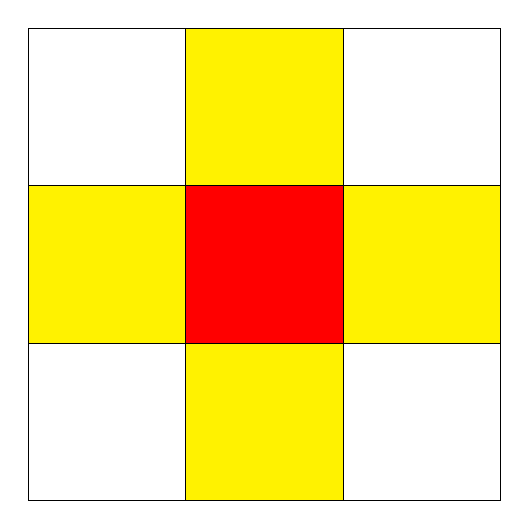
\begin{tikzpicture}
		\draw (0, 0) rectangle ++(6, 6);
		\filldraw[color=yellow, draw=black] (0, 2) rectangle ++(2, 2);
		\filldraw[color=yellow, draw=black] (2, 4) rectangle ++(2, 2);
		\filldraw[color=yellow, draw=black] (4, 2) rectangle ++(2, 2);
		\filldraw[color=yellow, draw=black] (2, 0) rectangle ++(2, 2);
		\filldraw (2, 2)[color=red, draw=black] rectangle ++(2, 2);
		\end{tikzpicture}
		\caption{四邻域}
	\end{minipage}
	\begin{minipage}{0.45\linewidth}
		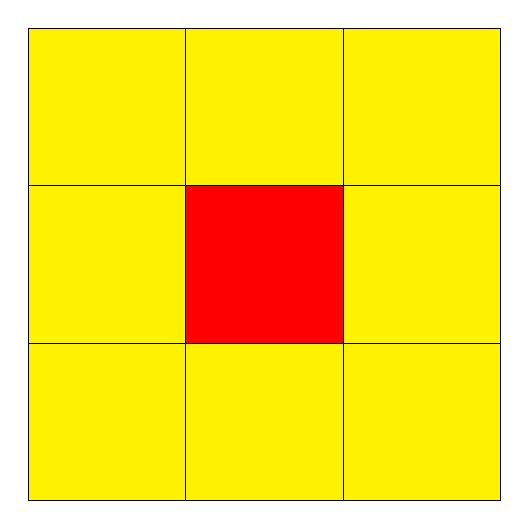
\begin{tikzpicture}
		\draw (0, 0) rectangle ++(6, 6);
		\filldraw (0, 0)[color=yellow, draw=black] rectangle ++(2, 2);
		\filldraw (0, 2)[color=yellow, draw=black] rectangle ++(2, 2);
		\filldraw (0, 4)[color=yellow, draw=black] rectangle ++(2, 2);
		\filldraw (2, 0)[color=yellow, draw=black] rectangle ++(2, 2);
		\filldraw (2, 2)[color=red, draw=black] rectangle ++(2, 2);
		\filldraw (2, 4)[color=yellow, draw=black] rectangle ++(2, 2);
		\filldraw (4, 0)[color=yellow, draw=black] rectangle ++(2, 2);
		\filldraw (4, 2)[color=yellow, draw=black] rectangle ++(2, 2);
		\filldraw (4, 4)[color=yellow, draw=black] rectangle ++(2, 2);
		\end{tikzpicture}
		\caption{八邻域}
	\end{minipage}
\end{figure}
\begin{description}
	\item[连通性] 两个像素是否连通取决于它们是否相邻以及它们的灰度值是否满足特定的相似性准则。
	\item[区域] 图像中的一个像素子集$\mathbb{R}$,该子集是一个连通集,则称$\mathbb{R}$为一个区域。
	\item[连通量] 具有相同输入值的邻接像素的区域。
	\item[连通分量的提取] 对每一个连通量,或每一个连通集$\mathbb{R}$赋予不同的标记。方便对$\mathbb{R}$进行分析。
	\item[$\mathbb{R}$的统计量] 面积,周长,质心,二阶矩等。最小外接矩形,$\mathbb{R}$区域的长度、宽度、长宽比。
\end{description}
\subsubsection{二值检测结果分析}
\begin{enumerate}
	\item 根据目标的大小,形状的先验知识,去除过大或过小的,形状不符合的连通区域。
	\item 对剩余的连通区域进行聚类,得到属于同一个目标的连通区域。
	\item 根据属于同一个目标的连通区域确定目标的中心。
	\item 以目标中心为中心切出目标候选切片。
	\item 进一步分析目标候选切片以去除虚警。
\end{enumerate}
连通区域聚类,得到属于同一个目标的连通区域。
\paragraph{层次聚类法}
\begin{enumerate}
	\item 每个连通区域自成一类,计算两辆距离,得到距离矩阵。
	\item 寻找距离最近的两个连通区域,划为一类。更新类别标记。
	\item 重新计算距离矩阵。
	\item 跳至步骤2,重复计算及合并。结束准则:最小距离大于一个阈值$T$。
\end{enumerate}
\subsection{实验流程}
\begin{figure}[H]
	\centering
	\begin{tikzpicture}[node distance=1.5cm]
	\node[startstop](begin){开始};
	\node[io, below of=begin](read_binarized_img){读取二值化判别图};
	\node[process, below of=read_binarized_img](label){标记连通区域};
	\node[process, below of=label](statistic){对连通区域计算质心、二阶矩};
	\node[process, below of=statistic](covariance){计算连通区域坐标协方差矩阵};
	\node[process, below of=covariance](area){计算连通区域面积};
	\node[process, below of=area](filte){筛选符合要求的目标};
	\node[process, below of=filte](mark_obj){在图片上标记目标};
	\node[io, below of=mark_obj](output){输出目标图像};
	\node[startstop, below of=output](end){结束};
	
	\draw[->] (begin) -- (read_binarized_img);
	\draw[->] (read_binarized_img) -- (label);
	\draw[->] (label) -- (statistic);
	\draw[->] (statistic) -- (covariance);
	\draw[->] (covariance) -- (area);
	\draw[->] (area) -- (filte);
	\draw[->] (filte) -- (mark_obj);
	\draw[->] (mark_obj) -- (output);
	\draw[->] (output) -- (end);
	\end{tikzpicture}
\end{figure}
\subsection{实验程序}
程序对不同连通分量的面积、质心、长宽比等参数进行计算,并依据面积和长宽比对目标进行筛选,以此筛选得到感兴趣对目标。
\lstinputlisting[caption={MarkBridge47.m}]{"../Executable Script/Exp 8/MarkBridge47.m"}
\lstinputlisting[caption={MarkBridge48.m}]{"../Executable Script/Exp 8/MarkBridge48.m"}
\lstinputlisting[caption={MarkBridge50.m}]{"../Executable Script/Exp 8/MarkBridge50.m"}
\lstinputlisting[caption={GetBinarizedImageObjectsInfo.m}]{"../Function Library/GetBinarizedImageObjectsInfo.m"}
\lstinputlisting[caption={DrawRectangle.m}]{"../Function Library/DrawRectangle.m"}
\lstinputlisting[caption={CutObjectsFromImage.m}]{"../Function Library/CutObjectsFromImage.m"}
\subsection{实验结果和分析}
\begin{figure}[H]
	\centering
	\begin{minipage}{0.45\linewidth}
		\includegraphics[width=\linewidth]{figure/bridge_47.jpg}
		\caption{bridge\_47原图}
	\end{minipage}
	\begin{minipage}{0.45\linewidth}
		\includegraphics[width=\linewidth]{figure/bridge_47_marked_ship.png}
		\caption{bridge\_47检测结果}
	\end{minipage}
\end{figure}
\begin{figure}[H]
	\centering
	\begin{minipage}{0.45\linewidth}
		\includegraphics[width=\linewidth]{figure/bridge_48.jpg}
		\caption{bridge\_48原图}
	\end{minipage}
	\begin{minipage}{0.45\linewidth}
		\includegraphics[width=\linewidth]{figure/bridge_48_marked_ship.png}
		\caption{bridge\_48检测结果}
	\end{minipage}
\end{figure}
\begin{figure}[H]
	\centering
	\begin{minipage}{0.45\linewidth}
		\includegraphics[width=\linewidth]{figure/bridge_50.jpg}
		\caption{bridge\_50原图}
	\end{minipage}
	\begin{minipage}{0.45\linewidth}
		\includegraphics[width=\linewidth]{figure/bridge_50_marked_ship.png}
		\caption{bridge\_50检测结果}
	\end{minipage}
\end{figure}
\begin{figure}[H]
	\centering
	\begin{minipage}{0.3\linewidth}
		\includegraphics[width=\linewidth]{figure/bridge_47_cutted_object_1.png}
	\end{minipage}
	\begin{minipage}{0.3\linewidth}
		\includegraphics[width=\linewidth]{figure/bridge_48_cutted_object_1.png}
	\end{minipage}
	\begin{minipage}{0.3\linewidth}
		\includegraphics[width=\linewidth]{figure/bridge_50_cutted_object_1.png}
	\end{minipage}
	\caption{从图中截取的船只}
\end{figure}
对检测结果进行标记和筛选后,根据先验知识,我们可以设定筛选出船只的条件,比如面积、长宽比等特征。根据这些条件,我们可以从有许多虚警的图片中,筛选出最有可能是船只的目标。从上图可以看出,根据设定的筛选条件,程序成功的从图片中选出了图片中的船只。